\section{Abläufe}

Während in Kapitel 3 die Interaktion der Hauptkomponenten Server und der RobotUnit abgehandelt wurden, werden im Folgenden die Abläufe der Use Cases genauer spezifiziert und auch interne Komponentenabläufe beschrieben, im Speziellen die Abläufe innerhalb der RobotUnit.

\subsection*{Use Cases in Wechselwirkung mit der IDrive Komponente }
Sobald der Roboter mit Perform Task(Usecase 2.2)  und Continue Task( Use Case  2.3) eingehende Aufgaben erhält, wird in jedem Fall das Ziel für die IDrive-Komponente spezifiziert. 
Und der Roboter setzt, sofern kein Abbruchanweisung dazwischenspielt, seinen Weg ungebrochen fort. Hat die IDrive-Komponente im Wechselspiel mit der INorthStar-Komponente für die räumliche Orientierung dann ihren Zielort erreicht, wird dies wiederum an die RobotUnit übermittelt, die weiter mit dem Server über ihre IWlanAdapter Komponene kommunzieren kann, wie es im UseCase ReceiveArrivalNotification( Use Case 1.5) der Fall ist.
\\

		\begin{figure}[H]
		\centering
		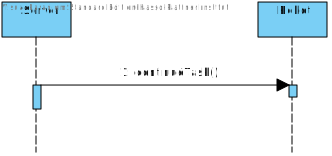
\includegraphics[width=1\textwidth]{img/2-Entwurf-ContinueTask}
		\caption{Sequenzdiagramm von \emph{Continue Task}}
		\label{ReadSensors}
	\end{figure}
	
	\begin{figure}[H]
		\centering
		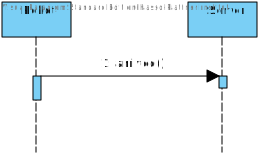
\includegraphics[width=1\textwidth]{img/2-Entwurf-ReceiveArrivalNotification}
		\caption{Sequenzdiagramm von \emph{ReceiveArrivalNotification}}
		\label{ReadSensors}
	\end{figure}

	\subsection*{Interaktion bei Ausführung von Use Case 2.1 – \emph{Read Sensors}}
In der folgenden Grafik wird der reine Informationsanfrageprozess zwischen Server und der RobotUnit dargestellt, auf dessen Basis ersterer alle notwendigen Daten über die zur Verfügung stehenden RobutUnits jederzeit abrufen kann; insbesondere wenn eine optimale Auswahl für ein Taxi oder einen Krankentransporter getroffen werden soll. 
Nach der Anfrage, wird die RobotUnit alle nötigen Informationen nacheinander abfragen: Sowohl die Position als auch die Orientierungsrichtung werden von der INorthStar-Komponente zurückgeliefert. 
Für den Batteriestatus muss die IBattery-Komponente angefragt werden. 
Erst wenn alle Informationen als Gesamtpaket bereitstehen, können sie an den Server zurückgemeldet werden.

\\

	\begin{figure}[H]
		\centering
		\includegraphics[width=1\textwidth]{img/0-Entwurf-8-ReadSens}
		\caption{Sequenzdiagramm von \emph{Read Sensors}}
		\label{ReadSensors}
	\end{figure}

	
	\subsection*{Interner Ablauf im Falle der Begegnung eines Hindernisses}}
	Sowohl die Methoden Path Around Obstacle als auch der Use Case Drive AroundObstacle sind beides Bestandteile des internen Ablauflaufprozesses, der im Falle eines auftauchenden Hindernisses einsetzt. 
	Die RobotUnit befindet sich dabei stets in einem Fahrvorgang, der stets konkret mit der Zielposition und er Geschwindigkeit vom Server eingestellt wurde. 
	So reagiert intern seine Software mit dem IDistanceSensor, wenn ein Hindernis um ihn herum auftaucht und dieses mit Hilfe der durch die Sensoren gesammelten Informationen umfahren werden muss. 
	Dabei muss der Roboter ausdrücklich zwischen einem Roboter und einem unbeweglichen Hindernis unterscheiden, um so vorherzubestimmen wie eine optimale Ausweichbewegung aussehen wird. 
	Auch wenn die IDistanceSensor die vollständige Umgebung um den Roboter wahrnehmen kann, bezieht sich dies jedoch primär auf vor dem Roboter liegende Hindernisse. 
	Dieser Prozess ist Bestandteil des Methode Choose Path around Obstacle und geht dann in den Methode Drive Around Obstacle über. 
	Der Roboter koordiniert sich dort mit seiner IDrive-Komponente und seinen Sensoren, um langsam an einem unbeweglichen Objekt vorbeizufahren. 
	Dabei fährt er immer eine kleine Distanz parallel zur Kante des Obstacles und prüft ob der Weg zur Destination wieder frei ist. 
	Ist dies der Fall nimmt er den Fahrtprozess wieder auf. 
	Erkennen sich zwei Roboter hingegen gegenseitig als Hindernis weichen beide mit Hilfe ihrer IDrive Komponente nach rechts aus, und nehmen anschließend den normalen Fahrbetrieb wieder auf. 
	Sollten all diese Vorkehrungen dennoch nicht helfen, setzt der IBumperHandler ein. 
	Dieser kann sofortig über den Server Request Repair( Use Case 1.6) anfordern oder im Falle das Passagiere an der Kollision beteiligt waren, einen Krankentransporter anrufen.
 \\
	
	\begin{figure}[H]
		\centering
		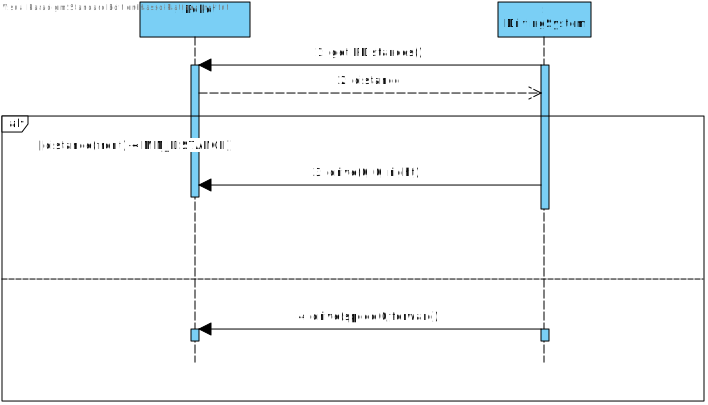
\includegraphics[width=0.95\textwidth]{img/1-Entwurf-8-DriveArroundObstacle}
		\caption{Sequenzdiagramm von \emph{Drive arround Obstacle}}
		\label{UmfahrenvonstatichenObjekten}
	\end{figure}
	\vspace{1cm}
	
	\subsection*{Interner Ablauf Charging}
	Charging ist eine Methode und ein spezieller interner Ablauf der RobotUnit für den keine weitere Kommunikation mit der Komponente Server stattfinden muss, dafür allerdings zwischen der RobotUnit und der ChargingStation. 
	Hat der Roboter einen bestimmten kritischen Ladestand erreicht(, den er regelmäßig überprüft), läuft er die ChargingStation-Komponente an. 
	Der Ladevorgang triggert automatische, sobald der Roboter die Position der Ladestation erreicht hat, und interagiert solange mit ihr bis seine Batterie wieder aufgeladen ist. 
	Innerhalb des Robots werden zum Anfahren der ChargingStation die Komponenten IBatterie mit der Position der Robotereigenen Ladestation und IDrive benötigt. 
	Konkret: Wenn IDrive arrived() zurückgibt, kann der Ladevorgang begonnen werden.
	\vspace{1cm}
	
	\begin{figure}[H]
		\centering
		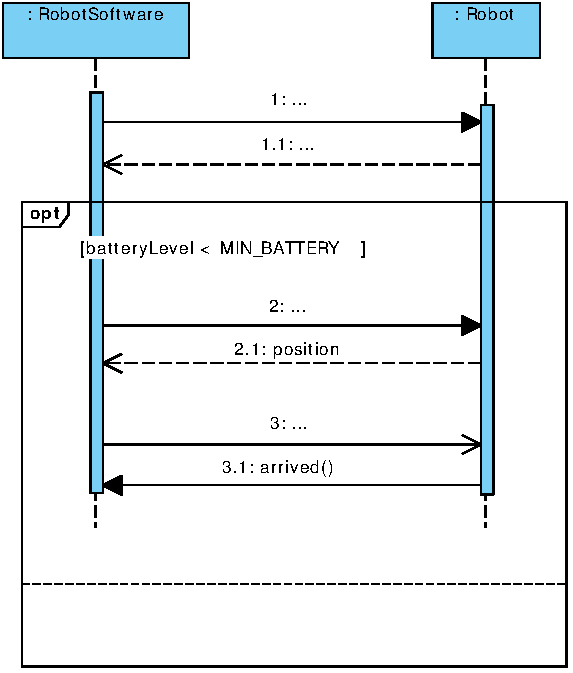
\includegraphics[width=0.65\textwidth]{img/0-Entwurf-8-Charging}
		\caption{Sequenzdiagramm von \textit{Charging}}
		\label{Charging}
	\end{figure}
